\item Con una hoja rectangular de cartón cuyas dimensiones son $12\text{ pulg}$ por $20\text{ pulg}$, se va a construir una caja abierta recortando cuadrados iguales de lado $x$ en cada una de las esquinas y luego doblando los bordes hacia arriba, como se ilustra en la figura. Exprese el volumen $V$ de la caja en función de $x$.
    
    \begin{center}
    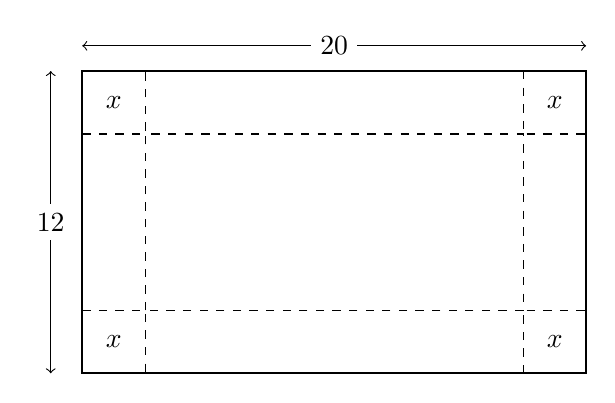
\begin{tikzpicture}[scale=0.8]
        % Rectángulo principal
        \draw[thick] (0,0) rectangle (8, 4.8);
        
        % Cortes en las esquinas
        \draw[dashed] (0, 3.8) -- (1, 3.8) -- (1, 4.8);
        \draw[dashed] (7, 4.8) -- (7, 3.8) -- (8, 3.8);
        \draw[dashed] (0, 1) -- (1, 1) -- (1, 0);
        \draw[dashed] (7, 0) -- (7, 1) -- (8, 1);
        
        % Líneas de doblez
        \draw[dashed] (1, 1) rectangle (7, 3.8);
        
        % Medidas
        \draw[<->] (0, 5.2) -- (8, 5.2) node[midway, fill=white] {20};
        \draw[<->] (-0.5, 0) -- (-0.5, 4.8) node[midway, fill=white] {12};
        
        \node at (0.5, 4.3) {$x$};
        \node at (0.5, 0.5) {$x$};
        \node at (7.5, 4.3) {$x$};
        \node at (7.5, 0.5) {$x$};
    \end{tikzpicture}
    \end{center}
